\documentclass[]{tufte-handout}

% ams
\usepackage{amssymb,amsmath}

\usepackage{ifxetex,ifluatex}
\usepackage{fixltx2e} % provides \textsubscript
\ifnum 0\ifxetex 1\fi\ifluatex 1\fi=0 % if pdftex
  \usepackage[T1]{fontenc}
  \usepackage[utf8]{inputenc}
\else % if luatex or xelatex
  \makeatletter
  \@ifpackageloaded{fontspec}{}{\usepackage{fontspec}}
  \makeatother
  \defaultfontfeatures{Ligatures=TeX,Scale=MatchLowercase}
  \makeatletter
  \@ifpackageloaded{soul}{
     \renewcommand\allcapsspacing[1]{{\addfontfeature{LetterSpace=15}#1}}
     \renewcommand\smallcapsspacing[1]{{\addfontfeature{LetterSpace=10}#1}}
   }{}
  \makeatother

\fi

% graphix
\usepackage{graphicx}
\setkeys{Gin}{width=\linewidth,totalheight=\textheight,keepaspectratio}

% booktabs
\usepackage{booktabs}

% url
\usepackage{url}

% hyperref
\usepackage{hyperref}

% units.
\usepackage{units}


\setcounter{secnumdepth}{-1}

% citations
\usepackage{natbib}
\bibliographystyle{plainnat}

% pandoc syntax highlighting

% longtable

% multiplecol
\usepackage{multicol}

% strikeout
\usepackage[normalem]{ulem}

% morefloats
\usepackage{morefloats}


% tightlist macro required by pandoc >= 1.14
\providecommand{\tightlist}{%
  \setlength{\itemsep}{0pt}\setlength{\parskip}{0pt}}

% title / author / date
\title{Try Bayesian Survival Analysis using the JACC study data
(traditional Cox-proportional hazard model presentations)}
\author{Chaochen Wang \textbar{} Aichi Medical University}
\date{2020-07-06}

\usepackage{booktabs}
\usepackage{longtable}
\usepackage{array}
\usepackage{multirow}
\usepackage{wrapfig}
\usepackage{float}
\usepackage{colortbl}
\usepackage{pdflscape}
\usepackage{tabu}
\usepackage{threeparttable}
\usepackage{threeparttablex}
\usepackage[normalem]{ulem}
\usepackage{makecell}
\usepackage{xcolor}

\begin{document}

\maketitle




\hypertarget{data-preparation}{%
\section{Data preparation}\label{data-preparation}}

Before exclusion, we have 110585 participants (46395 men and 64190
women) aged between 40-79 at baseline in the JACC data set:

\begin{verbatim}
## # A tibble: 2 x 3
##   tr_sex     n rel.freq
##   <chr>  <int> <chr>   
## 1 1      46395 41.95%  
## 2 2      64190 58.05%
\end{verbatim}

\hypertarget{excluding-participants-with-conditions}{%
\subsection{Excluding participants with
conditions}\label{excluding-participants-with-conditions}}

\begin{enumerate}
\def\labelenumi{\arabic{enumi}.}
\tightlist
\item
  With stroke history: n = 1496 (915 men and 581 wmen);
\item
  With cancer history: n = 1461 (411 men and 1050 women);
\item
  With myocardial infarction history: n = 2994 (1310 men and 1684
  women);
\item
  With ischemic heart diseases history: n = 186 (91 men, 95 women);
\item
  With other heart diseases history (ICD9 codes: 420-429): n = 518 (204
  men and 314 women);
\item
  Did not answer the question about milk intake frequency: n = 9545
  (3593 men and 5952 women);
\item
  Finally, n = 94385 (39386 men and 54999 women) are left in the data:
\end{enumerate}

\begin{verbatim}
## # A tibble: 6 x 4
## # Groups:   tr_sex [2]
##   tr_sex Tot_Stroke       n rel.freq
##   <chr>  <chr>        <int> <chr>   
## 1 1      Alive/Censor 27401 69.57%  
## 2 1      I60_9         1352 3.43%   
## 3 1      other_death  10633 27%     
## 4 2      Alive/Censor 45672 83.04%  
## 5 2      I60_9         1323 2.41%   
## 6 2      other_death   8004 14.55%
\end{verbatim}

\begin{itemize}
\tightlist
\item
  N of total stroke mortality (I60-I69) confirmed: 2675 (1352 men and
  1323 women) \newpage
\item
  Subtypes of stroke and CHD, heart failure:

  \begin{itemize}
  \tightlist
  \item
    Ischemic stroke: 957 (520 men and 437 women);
  \item
    Hemorrhagic stroke: 952 (432 men and 520 women);
  \item
    CHD: 1320 (749 men and 571 women);
  \item
    Heart failure: 1097 (498 men and 599 women).
  \end{itemize}
\item
  Follow-up years summary in total sample:
\end{itemize}

\begin{verbatim}
##  obs.  mean   median  s.d.   min.   max.  
##  94385 16.476 19.34   5.689  0.005  23.001
\end{verbatim}

\begin{itemize}
\tightlist
\item
  Follow-up years summary by total stroke mortality events:
\end{itemize}

\begin{verbatim}
## # A tibble: 6 x 6
## # Groups:   tr_sex [2]
##   tr_sex Tot_Stroke       n MeanFolYear MedianFolYear MaxFolYear
##   <chr>  <chr>        <int>       <dbl>         <dbl>      <dbl>
## 1 1      Alive/Censor 27401        18.1          20.3       23.0
## 2 1      I60_9         1352        11.2          11.1       22.9
## 3 1      other_death  10633        11.6          11.8       23.0
## 4 2      Alive/Censor 45672        17.7          20.1       23.0
## 5 2      I60_9         1323        11.8          11.9       22.9
## 6 2      other_death   8004        12.4          13.1       23.0
\end{verbatim}

\begin{figure}

{\centering 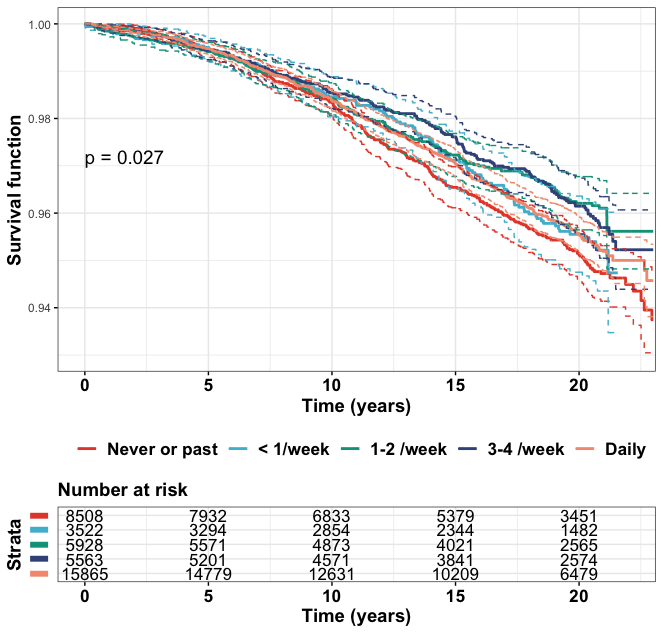
\includegraphics[width=0.95\linewidth]{fig/KMfigMen} 

}

\caption[Kaplan-Meier survival curves for total stroke mortality by milk drinking frequency (P value was obtained from log-rank tests) in men]{Kaplan-Meier survival curves for total stroke mortality by milk drinking frequency (P value was obtained from log-rank tests) in men.}\label{fig:KMmen}
\end{figure}

\begin{figure}

{\centering 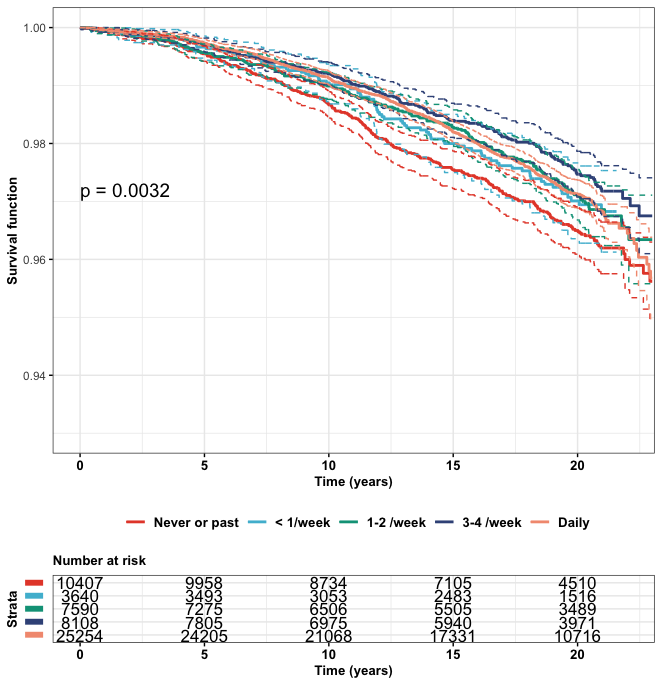
\includegraphics[width=0.9\linewidth]{fig/KMfigwomen} 

}

\caption[Kaplan-Meier survival curves for total stroke mortality by milk drinking frequency (P value was obtained from log-rank tests) in women]{Kaplan-Meier survival curves for total stroke mortality by milk drinking frequency (P value was obtained from log-rank tests) in women.}\label{fig:KMwomen}
\end{figure}

\newpage

\begin{table}[!htbp]

Table 1. Baseline characteristics of subjects in the JACC study by milk intake level in Men (n = 39,386).

\centering
\fontsize{8}{10}\selectfont
\begin{tabular}[t]{llllllll}
\toprule
\multicolumn{1}{c}{ } & \multicolumn{1}{c}{} & \multicolumn{1}{c}{} & \multicolumn{4}{c}{Milk drinkers} & \multicolumn{1}{c}{} \\
\cmidrule(l{3pt}r{3pt}){4-7}
Characteristic & Never & Drinker & 1-2 t/Mon & 1-2 t/Week & 3-4 t/Week & Daily & P value\\
\midrule
\rowcolor{gray!6}  n & 8508 & 30878 & 3522 & 5928 & 5563 & 15865 & \\
Age (mean (SD)) & 56.80 (9.97) & 56.78 (10.15) & 55.18 (10.14) & 55.42 (10.10) & 55.43 (9.95) & 58.12 (10.07) & <0.001\\
\rowcolor{gray!6}  Smoking (\%) &  &  &  &  &  &  & <0.001\\
\hspace{1em}Never & 1384 (16.3) & 6479 (21.0) & 652 (18.5) & 1091 (18.4) & 1141 (20.5) & 3595 (22.7) & \\
\rowcolor{gray!6}  \hspace{1em}Past & 1836 (21.6) & 7729 (25.0) & 730 (20.7) & 1298 (21.9) & 1335 (24.0) & 4366 (27.5) & \\
\hspace{1em}Current & 4996 (58.7) & 15386 (49.8) & 2020 (57.4) & 3313 (55.9) & 2845 (51.1) & 7208 (45.4) & \\
\rowcolor{gray!6}  Alc\_Fre (\%) &  &  &  &  &  &  & <0.001\\
\hspace{1em}< 1/week & 355 ( 4.2) & 1469 ( 4.8) & 130 ( 3.7) & 273 ( 4.6) & 301 ( 5.4) & 765 ( 4.8) & \\
\rowcolor{gray!6}  \hspace{1em}1-4 /week & 1105 (13.0) & 5316 (17.2) & 597 (17.0) & 1056 (17.8) & 1033 (18.6) & 2630 (16.6) & \\
\hspace{1em}Daily & 4416 (51.9) & 14746 (47.8) & 1793 (50.9) & 2871 (48.4) & 2706 (48.6) & 7376 (46.5) & \\
\rowcolor{gray!6}  \hspace{1em}Never or past & 2028 (23.8) & 7060 (22.9) & 727 (20.6) & 1257 (21.2) & 1120 (20.1) & 3956 (24.9) & \\
BMI (mean (SD)) & 22.58 (3.41) & 22.71 (3.41) & 22.76 (2.75) & 22.76 (2.82) & 22.91 (5.44) & 22.61 (2.75) & <0.001\\
\rowcolor{gray!6}  BMIgrp (\%) &  &  &  &  &  &  & <0.001\\
\hspace{1em}18.5-24.9 & 6099 (71.7) & 22591 (73.2) & 2562 (72.7) & 4313 (72.8) & 4042 (72.7) & 11674 (73.6) & \\
\rowcolor{gray!6}  \hspace{1em}< 18.5 & 505 ( 5.9) & 1446 ( 4.7) & 152 ( 4.3) & 266 ( 4.5) & 213 ( 3.8) & 815 ( 5.1) & \\
\hspace{1em}25-29.9 & 1404 (16.5) & 5246 (17.0) & 612 (17.4) & 1082 (18.3) & 988 (17.8) & 2564 (16.2) & \\
\rowcolor{gray!6}  \hspace{1em}> 30 & 90 ( 1.1) & 296 ( 1.0) & 38 ( 1.1) & 54 ( 0.9) & 63 ( 1.1) & 141 ( 0.9) & \\
Exercise (\%) &  &  &  &  &  &  & <0.001\\
\rowcolor{gray!6}  \hspace{1em}Almost0 & 5009 (58.9) & 17232 (55.8) & 2274 (64.6) & 3316 (55.9) & 2954 (53.1) & 8688 (54.8) & \\
\hspace{1em}> 1h/w & 1618 (19.0) & 8509 (27.6) & 934 (26.5) & 1482 (25.0) & 1418 (25.5) & 4675 (29.5) & \\
\rowcolor{gray!6}  Slepgrp (\%) &  &  &  &  &  &  & <0.001\\
\hspace{1em}< 6.9 & 1502 (17.7) & 5274 (17.1) & 582 (16.5) & 1036 (17.5) & 948 (17.0) & 2708 (17.1) & \\
\rowcolor{gray!6}  \hspace{1em}7-7.9 & 2559 (30.1) & 9953 (32.2) & 1182 (33.6) & 1891 (31.9) & 1802 (32.4) & 5078 (32.0) & \\
\hspace{1em}8-8.9 & 3026 (35.6) & 11074 (35.9) & 1217 (34.6) & 2143 (36.2) & 1953 (35.1) & 5761 (36.3) & \\
\rowcolor{gray!6}  \hspace{1em}> 9 & 1113 (13.1) & 3102 (10.0) & 374 (10.6) & 581 ( 9.8) & 553 ( 9.9) & 1594 (10.0) & \\
Veg (\%) &  &  &  &  &  &  & <0.001\\
\rowcolor{gray!6}  \hspace{1em}Less1tm & 1002 (11.8) & 2556 ( 8.3) & 556 (15.8) & 508 ( 8.6) & 362 ( 6.5) & 1130 ( 7.1) & \\
\hspace{1em}One2tw & 2198 (25.8) & 7915 (25.6) & 1118 (31.7) & 1828 (30.8) & 1280 (23.0) & 3689 (23.3) & \\
\rowcolor{gray!6}  \hspace{1em}Thre4tw & 1787 (21.0) & 7791 (25.2) & 871 (24.7) & 1333 (22.5) & 1582 (28.4) & 4005 (25.2) & \\
\hspace{1em}daily & 1810 (21.3) & 7844 (25.4) & 709 (20.1) & 1209 (20.4) & 1158 (20.8) & 4768 (30.1) & \\
\rowcolor{gray!6}  Fruit (\%) &  &  &  &  &  &  & <0.001\\
\hspace{1em}Less1tm & 1888 (22.2) & 4007 (13.0) & 786 (22.3) & 810 (13.7) & 618 (11.1) & 1793 (11.3) & \\
\rowcolor{gray!6}  \hspace{1em}One2tw & 1877 (22.1) & 6691 (21.7) & 999 (28.4) & 1581 (26.7) & 1099 (19.8) & 3012 (19.0) & \\
\hspace{1em}Thre4tw & 1376 (16.2) & 6120 (19.8) & 695 (19.7) & 1122 (18.9) & 1271 (22.8) & 3032 (19.1) & \\
\rowcolor{gray!6}  \hspace{1em}daily & 1260 (14.8) & 6924 (22.4) & 542 (15.4) & 968 (16.3) & 961 (17.3) & 4453 (28.1) & \\
Greentea (\%) &  &  &  &  &  &  & <0.001\\
\rowcolor{gray!6}  \hspace{1em}daily & 6508 (76.5) & 24444 (79.2) & 2814 (79.9) & 4641 (78.3) & 4332 (77.9) & 12657 (79.8) & \\
\hspace{1em}Thre3tw & 737 ( 8.7) & 2926 ( 9.5) & 378 (10.7) & 588 ( 9.9) & 562 (10.1) & 1398 ( 8.8) & \\
\rowcolor{gray!6}  \hspace{1em}Never & 659 ( 7.7) & 1748 ( 5.7) & 184 ( 5.2) & 327 ( 5.5) & 299 ( 5.4) & 938 ( 5.9) & \\
Coffe (\%) &  &  &  &  &  &  & <0.001\\
\rowcolor{gray!6}  \hspace{1em}daily & 3727 (43.8) & 15662 (50.7) & 1780 (50.5) & 2845 (48.0) & 2642 (47.5) & 8395 (52.9) & \\
\hspace{1em}Thre3tw & 2267 (26.6) & 8511 (27.6) & 998 (28.3) & 1822 (30.7) & 1774 (31.9) & 3917 (24.7) & \\
\rowcolor{gray!6}  \hspace{1em}Never & 2299 (27.0) & 6006 (19.5) & 700 (19.9) & 1123 (18.9) & 983 (17.7) & 3200 (20.2) & \\
Educgrp (\%) &  &  &  &  &  &  & <0.001\\
\rowcolor{gray!6}  \hspace{1em}>= 18 y.o & 2168 (25.5) & 10701 (34.7) & 1190 (33.8) & 1973 (33.3) & 1726 (31.0) & 5812 (36.6) & \\
DM\_hist (\%) &  &  &  &  &  &  & <0.001\\
\rowcolor{gray!6}  \hspace{1em}TRUE & 423 ( 5.0) & 1942 ( 6.3) & 160 ( 4.5) & 250 ( 4.2) & 304 ( 5.5) & 1228 ( 7.7) & \\
HT\_hist (\%) &  &  &  &  &  &  & 0.039\\
\rowcolor{gray!6}  \hspace{1em}TRUE & 1568 (18.4) & 5526 (17.9) & 616 (17.5) & 1013 (17.1) & 937 (16.8) & 2960 (18.7) & \\
KID\_hist (\%) &  &  &  &  &  &  & <0.001\\
\rowcolor{gray!6}  \hspace{1em}TRUE & 257 ( 3.0) & 1038 ( 3.4) & 135 ( 3.8) & 178 ( 3.0) & 168 ( 3.0) & 557 ( 3.5) & \\
LIV\_hist (\%) &  &  &  &  &  &  & <0.001\\
\rowcolor{gray!6}  \hspace{1em}TRUE & 495 ( 5.8) & 2016 ( 6.5) & 223 ( 6.3) & 356 ( 6.0) & 300 ( 5.4) & 1137 ( 7.2) & \\
\bottomrule
\multicolumn{8}{l}{\textit{Note: }}\\
\multicolumn{8}{l}{Abbreviations: n, number; SD, standard deviation; Alc\_Fre, alcohol intake; BMI, Body Mass Index; Slepgrp, sleep duration}\\
\multicolumn{8}{l}{groups; Veg, vegetable intake; Coffe, coffee intake; DM/HT/KID/LIV\_hist, diabetes, hypertension, kidney disease,}\\
\multicolumn{8}{l}{liver disease history.}\\
\end{tabular}
\end{table}

\newpage

\begin{table}[!htbp]
Table 2. Baseline characteristics of subjects in the JACC study by milk intake level in Women (n = 54,999).

\centering
\fontsize{8}{10}\selectfont
\begin{tabular}[t]{llllllll}
\toprule
\multicolumn{1}{c}{ } & \multicolumn{1}{c}{} & \multicolumn{1}{c}{} & \multicolumn{4}{c}{Milk drinkers} & \multicolumn{1}{c}{} \\
\cmidrule(l{3pt}r{3pt}){4-7}
Characteristic & Never & Drinker & 1-2 t/Mon & 1-2 t/Week & 3-4 t/Week & Daily & P value\\
\midrule
\rowcolor{gray!6}  n & 10407 & 44592 & 3640 & 7590 & 8108 & 25254 & \\
Age (mean (SD)) & 58.03 (10.17) & 56.97 (9.99) & 56.52 (10.19) & 55.60 (10.08) & 55.58 (9.89) & 57.90 (9.86) & <0.001\\
\rowcolor{gray!6}  Smoking (\%) &  &  &  &  &  &  & <0.001\\
\hspace{1em}Never & 8318 (79.9) & 36978 (82.9) & 2974 (81.7) & 6219 (81.9) & 6763 (83.4) & 21022 (83.2) & \\
\rowcolor{gray!6}  \hspace{1em}Past & 169 ( 1.6) & 607 ( 1.4) & 49 ( 1.3) & 113 ( 1.5) & 98 ( 1.2) & 347 ( 1.4) & \\
\hspace{1em}Current & 723 ( 6.9) & 1860 ( 4.2) & 222 ( 6.1) & 420 ( 5.5) & 346 ( 4.3) & 872 ( 3.5) & \\
\rowcolor{gray!6}  Alc\_Fre (\%) &  &  &  &  &  &  & <0.001\\
\hspace{1em}< 1/week & 697 ( 6.7) & 3084 ( 6.9) & 191 ( 5.2) & 567 ( 7.5) & 673 ( 8.3) & 1653 ( 6.5) & \\
\rowcolor{gray!6}  \hspace{1em}1-4 /week & 837 ( 8.0) & 4611 (10.3) & 357 ( 9.8) & 828 (10.9) & 918 (11.3) & 2508 ( 9.9) & \\
\hspace{1em}Daily & 450 ( 4.3) & 2021 ( 4.5) & 200 ( 5.5) & 325 ( 4.3) & 338 ( 4.2) & 1158 ( 4.6) & \\
\rowcolor{gray!6}  \hspace{1em}Never or past & 7449 (71.6) & 30670 (68.8) & 2562 (70.4) & 5196 (68.5) & 5416 (66.8) & 17496 (69.3) & \\
BMI (mean (SD)) & 23.01 (3.38) & 22.91 (3.69) & 23.02 (3.80) & 23.07 (4.41) & 23.07 (3.08) & 22.80 (3.62) & <0.001\\
\rowcolor{gray!6}  BMIgrp (\%) &  &  &  &  &  &  & <0.001\\
\hspace{1em}18.5-24.9 & 6589 (63.3) & 30588 (68.6) & 2438 (67.0) & 5121 (67.5) & 5496 (67.8) & 17533 (69.4) & \\
\rowcolor{gray!6}  \hspace{1em}< 18.5 & 703 ( 6.8) & 2465 ( 5.5) & 188 ( 5.2) & 380 ( 5.0) & 398 ( 4.9) & 1499 ( 5.9) & \\
\hspace{1em}25-29.9 & 2173 (20.9) & 8545 (19.2) & 756 (20.8) & 1505 (19.8) & 1678 (20.7) & 4606 (18.2) & \\
\rowcolor{gray!6}  \hspace{1em}> 30 & 280 ( 2.7) & 769 ( 1.7) & 76 ( 2.1) & 175 ( 2.3) & 158 ( 1.9) & 360 ( 1.4) & \\
Exercise (\%) &  &  &  &  &  &  & <0.001\\
\rowcolor{gray!6}  \hspace{1em}Almost0 & 6618 (63.6) & 27513 (61.7) & 2624 (72.1) & 4816 (63.5) & 4790 (59.1) & 15283 (60.5) & \\
\hspace{1em}> 1h/w & 1417 (13.6) & 9265 (20.8) & 624 (17.1) & 1401 (18.5) & 1522 (18.8) & 5718 (22.6) & \\
\rowcolor{gray!6}  Slepgrp (\%) &  &  &  &  &  &  & <0.001\\
\hspace{1em}< 6.9 & 2805 (27.0) & 11968 (26.8) & 1019 (28.0) & 2047 (27.0) & 2103 (25.9) & 6799 (26.9) & \\
\rowcolor{gray!6}  \hspace{1em}7-7.9 & 3336 (32.1) & 16071 (36.0) & 1245 (34.2) & 2721 (35.8) & 2944 (36.3) & 9161 (36.3) & \\
\hspace{1em}8-8.9 & 2886 (27.7) & 11432 (25.6) & 914 (25.1) & 1965 (25.9) & 2056 (25.4) & 6497 (25.7) & \\
\rowcolor{gray!6}  \hspace{1em}> 9 & 887 ( 8.5) & 2543 ( 5.7) & 254 ( 7.0) & 439 ( 5.8) & 435 ( 5.4) & 1415 ( 5.6) & \\
Veg (\%) &  &  &  &  &  &  & <0.001\\
\rowcolor{gray!6}  \hspace{1em}Less1tm & 917 ( 8.8) & 2356 ( 5.3) & 399 (11.0) & 445 ( 5.9) & 337 ( 4.2) & 1175 ( 4.7) & \\
\hspace{1em}One2tw & 2514 (24.2) & 10127 (22.7) & 1029 (28.3) & 2195 (28.9) & 1642 (20.3) & 5261 (20.8) & \\
\rowcolor{gray!6}  \hspace{1em}Thre4tw & 2331 (22.4) & 11845 (26.6) & 1001 (27.5) & 1876 (24.7) & 2452 (30.2) & 6516 (25.8) & \\
\hspace{1em}daily & 2567 (24.7) & 13537 (30.4) & 909 (25.0) & 1866 (24.6) & 1963 (24.2) & 8799 (34.8) & \\
\rowcolor{gray!6}  Fruit (\%) &  &  &  &  &  &  & <0.001\\
\hspace{1em}Less1tm & 1397 (13.4) & 3270 ( 7.3) & 523 (14.4) & 594 ( 7.8) & 514 ( 6.3) & 1639 ( 6.5) & \\
\rowcolor{gray!6}  \hspace{1em}One2tw & 1913 (18.4) & 6761 (15.2) & 801 (22.0) & 1515 (20.0) & 1122 (13.8) & 3323 (13.2) & \\
\hspace{1em}Thre4tw & 1926 (18.5) & 9018 (20.2) & 845 (23.2) & 1591 (21.0) & 1922 (23.7) & 4660 (18.5) & \\
\rowcolor{gray!6}  \hspace{1em}daily & 2601 (25.0) & 15939 (35.7) & 967 (26.6) & 2216 (29.2) & 2369 (29.2) & 10387 (41.1) & \\
Greentea (\%) &  &  &  &  &  &  & <0.001\\
\rowcolor{gray!6}  \hspace{1em}daily & 7680 (73.8) & 34264 (76.8) & 2804 (77.0) & 5800 (76.4) & 6146 (75.8) & 19514 (77.3) & \\
\hspace{1em}Thre3tw & 946 ( 9.1) & 4615 (10.3) & 394 (10.8) & 848 (11.2) & 921 (11.4) & 2452 ( 9.7) & \\
\rowcolor{gray!6}  \hspace{1em}Never & 944 ( 9.1) & 2928 ( 6.6) & 230 ( 6.3) & 467 ( 6.2) & 466 ( 5.7) & 1765 ( 7.0) & \\
Coffe (\%) &  &  &  &  &  &  & <0.001\\
\rowcolor{gray!6}  \hspace{1em}daily & 4121 (39.6) & 21483 (48.2) & 1682 (46.2) & 3519 (46.4) & 3597 (44.4) & 12685 (50.2) & \\
\hspace{1em}Thre3tw & 2648 (25.4) & 12514 (28.1) & 1069 (29.4) & 2279 (30.0) & 2698 (33.3) & 6468 (25.6) & \\
\rowcolor{gray!6}  \hspace{1em}Never & 3387 (32.5) & 9670 (21.7) & 835 (22.9) & 1611 (21.2) & 1620 (20.0) & 5604 (22.2) & \\
Educgrp (\%) &  &  &  &  &  &  & <0.001\\
\rowcolor{gray!6}  \hspace{1em}>= 18 y.o & 2073 (19.9) & 14092 (31.6) & 1016 (27.9) & 2263 (29.8) & 2225 (27.4) & 8588 (34.0) & \\
DM\_hist (\%) &  &  &  &  &  &  & <0.001\\
\rowcolor{gray!6}  \hspace{1em}TRUE & 269 ( 2.6) & 1642 ( 3.7) & 115 ( 3.2) & 206 ( 2.7) & 219 ( 2.7) & 1102 ( 4.4) & \\
HT\_hist (\%) &  &  &  &  &  &  & <0.001\\
\rowcolor{gray!6}  \hspace{1em}TRUE & 2236 (21.5) & 8782 (19.7) & 745 (20.5) & 1446 (19.1) & 1533 (18.9) & 5058 (20.0) & \\
KID\_hist (\%) &  &  &  &  &  &  & <0.001\\
\rowcolor{gray!6}  \hspace{1em}TRUE & 371 ( 3.6) & 1830 ( 4.1) & 142 ( 3.9) & 280 ( 3.7) & 298 ( 3.7) & 1110 ( 4.4) & \\
LIV\_hist (\%) &  &  &  &  &  &  & <0.001\\
\rowcolor{gray!6}  \hspace{1em}TRUE & 365 ( 3.5) & 2047 ( 4.6) & 178 ( 4.9) & 295 ( 3.9) & 320 ( 3.9) & 1254 ( 5.0) & \\
Menopause (\%) &  &  &  &  &  &  & <0.001\\
\rowcolor{gray!6}  \hspace{1em}TRUE & 8213 (78.9) & 34021 (76.3) & 2684 (73.7) & 5408 (71.3) & 5791 (71.4) & 20138 (79.7) & \\
\bottomrule
\multicolumn{8}{l}{\textit{Note: }}\\
\multicolumn{8}{l}{Abbreviations: n, number; SD, standard deviation; Alc\_Fre, alcohol intake; BMI, Body Mass Index; Slepgrp, sleep duration}\\
\multicolumn{8}{l}{groups; Veg, vegetable intake; Coffe, coffee intake; DM/HT/KID/LIV\_hist, diabetes, hypertension, kidney disease,}\\
\multicolumn{8}{l}{liver disease history.}\\
\end{tabular}
\end{table}

\begin{table}[!htbp]
Table 3. Sex-specific hazard ratio (95\% CI) of mortality from stroke according to milk intake frequency.

\centering
\fontsize{9}{11}\selectfont
\begin{tabular}[t]{llllll}
\toprule
 & Never & 1-2 t/Mon & 1-2 t/Week & 3-4 t/Week & Daily\\
\midrule
\rowcolor{gray!6}  Men &  &  &  &  & \\
N & 8508 & 3522 & 5928 & 5563 & 15865\\
\rowcolor{gray!6}  Person year & 135704 & 56551 & 97098 & 92153 & 252364\\
Total Stroke &  &  &  &  \vphantom{1} & \\
\rowcolor{gray!6}  \hspace{1em}n & 326 & 122 & 181 & 177 & 546\\
\hspace{1em}Crude model & 1 & 0.89 (0.73, 1.11) & 0.77 (0.64, 0.92) & 0.79 (0.66, 0.95) & 0.90 (0.79, 1.04)\\
\rowcolor{gray!6}  \hspace{1em}Age-adjusted & 1 & 0.99 (0.80, 1.22) & 0.84 (0.70, 1.01) & 0.86 (0.72, 1.03) & 0.76 (0.66, 0.87)\\
\hspace{1em}Multivariable-adjusted & 1 & 1.03 (0.83, 1.27) & 0.91 (0.75, 1.09) & 0.96 (0.79, 1.16) & 0.87 (0.76, 1.01)\\
\rowcolor{gray!6}  Hemorrhagic stroke &  &  &  &  \vphantom{1} & \\
\hspace{1em}n & 100 & 42 & 58 & 56 & 176\\
\rowcolor{gray!6}  \hspace{1em}Crude model & 1 & 1.00 (0.70, 1.44) & 0.81 (0.58, 1.11) & 0.82 (0.59, 1.14) & 0.94 (0.74, 1.21)\\
\hspace{1em}Age-adjusted & 1 & 1.07 (0.75, 1.55) & 0.86 (0.62, 1.19) & 0.87 (0.63, 1.21) & 0.85 (0.66, 1.08)\\
\rowcolor{gray!6}  \hspace{1em}Multivariable-adjusted & 1 & 1.11 (0.77, 1.60) & 0.94 (0.68, 1.31) & 1.01 (0.72, 1.40) & 0.98 (0.76, 1.27)\\
Ischemic stroke &  &  &  &  \vphantom{1} & \\
\rowcolor{gray!6}  \hspace{1em}n & 151 & 41 & 64 & 66 & 198\\
\hspace{1em}Crude model & 1 & 0.65 (0.46. 0.92) & 0.59 (0.44, 0.79) & 0.63 (0.48, 0.85) & 0.71 (0.57, 0.88)\\
\rowcolor{gray!6}  \hspace{1em}Age-adjusted & 1 & 0.73 (0.52, 1.03) & 0.65 (0.49, 0.87) & 0.70 (0.53, 0.94) & 0.58 (0.47, 0.72)\\
\hspace{1em}Multivariable-adjusted & 1 & 0.73 (0.51, 1.04) & 0.67 (0.49, 0.90) & 0.74 (0.55, 0.99) & 0.63 (0.50, 0.79)\\
\rowcolor{gray!6}  Women &  &  &  &  & \\
N & 10407 & 3640 & 7590 & 8108 & 25254\\
\rowcolor{gray!6}  Person year & 173222 & 59904 & 129233 & 139919 & 418925\\
Total Stroke &  &  &  &  & \\
\rowcolor{gray!6}  \hspace{1em}n & 300 & 84 & 182 & 172 & 585\\
\hspace{1em}Crude model & 1 & 0.83 (0.65, 1.05) & 0.81 (0.67, 0.97) & 0.69 (0.58, 0.84) & 0.81 (0.71, 0.93)\\
\rowcolor{gray!6}  \hspace{1em}Age-adjusted & 1 & 1.01 (0.79, 1.28) & 1.07 (0.89, 1.28) & 0.94 (0.78, 1.13) & 0.88 (0.77, 1.01)\\
\hspace{1em}Multivariable-adjusted & 1 & 1.05 (0.82, 1.34) & 1.12 (0.93, 1.35) & 1.01 (0.83, 1.22) & 0.99 (0.86, 1.15)\\
\rowcolor{gray!6}  Hemorrhagic stroke &  &  &  &  & \\
\hspace{1em}n & 108 & 27 & 78 & 76 & 231\\
\rowcolor{gray!6}  \hspace{1em}Crude model & 1 & 0.73 (0.48, 1.12) & 0.96 (0.72, 1.29) & 0.86 (0.64, 1.16) & 0.89 (0.71, 1.12)\\
\hspace{1em}Age-adjusted & 1 & 0.83 (0.54, 1.26) & 1.16 (0.86, 1.55) & 1.04 (0.77, 1.39) & 0.92 (0.73, 1.15)\\
\rowcolor{gray!6}  \hspace{1em}Multivariable-adjusted & 1 & 0.85 (0.56, 1.30) & 1.21 (0.90, 1.62) & 1.13 (0.84, 1.52) & 1.03 (0.81, 1.29)\\
Ischemic stroke &  &  &  &  & \\
\rowcolor{gray!6}  \hspace{1em}n & 102 & 35 & 63 & 50 & 187\\
\hspace{1em}Crude model & 1 & 1.01 (0.69, 1.48) & 0.82 (0.60, 1.13) & 0.59 (0.43, 0.84) & 0.76 (0.59, 0.97)\\
\rowcolor{gray!6}  \hspace{1em}Age-adjusted & 1 & 1.29 (0.88, 1.89) & 1.15 (0.84, 1.58) & 0.86 (0.61, 1.20) & 0.86 (0.67, 1.09)\\
\hspace{1em}Multivariable-adjusted & 1 & 1.30 (0.88, 1.92) & 1.18 (0.86, 1.63) & 0.87 (0.62, 1.23) & 0.93 (0.72, 1.19)\\
\bottomrule
\end{tabular}
\end{table}

\bibliography{skeleton.bib}



\end{document}
